\chapter{Context\label{section:context}}

% As of today little work has been done on creating a multihop LoRa Network (see Kris Paper on RPL LoRa in context section)
I will introduce in this chapter all the concepts needed for the understanding
of the experiment I conducted in this thesis.
I will also give an overview of related work to the topic.

\section{Low Power Wide Area Network (LPWAN)\label{section:lpwan}}

Every IoT project has its own requirements. 
LPWAN is typically made for sensor networks with limited throughput.
The characteristics of an LPWAN are the following.

\begin{itemize}
  \item Low power as the name suggest. The network is made of battery-operated
    motes that must run for years without replacement.
  \item Long range. Mote should transmit over multiple km without a repeater.
  \item Low cost devices. No expensive infrastructure requirement and motes
    operate with simple hardware.
  \item Limited data throughput.
\end{itemize}

LPWAN includes LoRa but it's not the only option available. 
Sigfox, NB-IOT are other well known LPWAN options.

\paragraph{IPv6 over Low-Power Wireless Personal Area Networks (6LoWPAN)}

6LoWPAN is an open standard defined in RFC 6282 by the Internet Engineering
Task Force (IETF).
The idea of 6LoWPAN is to bring IPv6 packet over the small link layer frame of
LPWAN with the help of a header compression mechanisms.
6LoWPAN brings native IP communication to LPWAN.
This means each mote of the network can now communicate simply using an
edge router that handles the data exchange between the 6LoWPAN network and the
internet.

\paragraph{6TiSCH}

In the same way as with 6LoWPAN, 6TiSCH defines an adaptation layer for IPv6
over TSCH named 6top.

\section{LoRa\label{section:lora}}

LoRa is a proprietary chirp spread spectrum technology made by Semtech with
integrated Forward Error Correction (FEC).
LoRa operates in this sub-GHz unlicensed Industrial, Scientific, and Medical
(ISM) bands.
The main characteristic of LoRa, is that it trades data rate for long-range 
and low-power consumption with a maximum data rate of 27 kbps~\cite{8030482}.
LoRa supports bi-directional communications with a maximum payload size of 242
bytes~\cite{loraalliance:lorawanspecification}.

This section will cover the LoRa physical layer parameters, the packet structure and 
will explain how all these parameters influence the Time On Air (ToA).

\subsection{Chirp Spread Spectrum (CSS) modulation}

Chirp Spread Spectrum is a spread spectrum technique, developed in 1940 for
military applications in radars and sonars \cite{semtech:modulationbasics}, but
has been adopted in recent years for low power data transmission.
Chirps are sinusoidal signals increasing (upchirps) or decreasing (downchirps)
in frequency over time.
Figure~\ref{fig:downchirp} shows an example of a downchirp.

Using CSS has the advantage of offering equivalent timing and frequency offset
between the receiver and transmitter and robustness to channel degradation
mechanisms (multipath, fading, Doppler, in-band jamming
interference)~\cite{semtech:modulationbasics}.

\tikzset{declare function={f(\x)=sin(540*\x);}}

\begin{figure}[H]
\centering
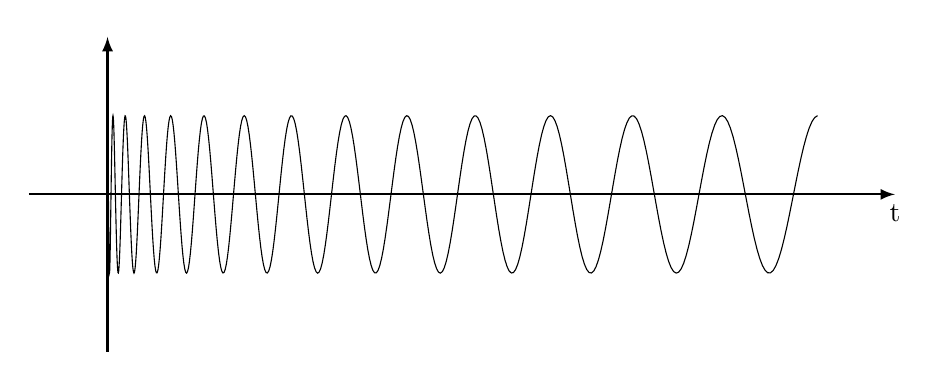
\begin{tikzpicture}
  \draw[thick,-latex] (0,-2) -- (0,2)node[right] {};
  \draw[thick,-latex] (-1,0) -- (10,0)node[below] {t};
  \draw[domain=0.1:9.5,variable=\x,samples=500] plot ({0.10*\x*\x}, {f(\x)});
\end{tikzpicture} 
\caption{Downchirp example\label{fig:downchirp}}
\end{figure}

\subsection{PHY Parameters}

% TODO remainder of why we do this ? explain those characteristics will be
% important in the TSCH implementation

\subsubsection{Spreading Factor (SF)}

The spreading factor, a parameter of the LoRa modulation, represents the
relation~(\ref{eq:sf}) between the symbol rate ($R_{s}$) and chirp rate ($R_{c}$)
(see~\cite{semtech:modemdesign}) where $2^{SF}$ equals to the number of chirps per
symbols.

\begin{equation}
 \label{eq:sf} 
  2^{SF} = \frac{R_c}{R_s}
\end{equation}

The SF can range from 7 to 12, higher SF improves the Signal-to-noise ratio
(SNR) and receiver sensitivity~\cite{semtech:modemdesign}.
Increasing the SF trades data rate for transmission range.

The LoRa modulation uses orthogonal spreading factors to enable concurrent
packet transmission at the same time with different
spreading factors~\cite{semtech:modulationbasics}.

\subsubsection{Bandwidth (BW)}

Bandwidth is the range of frequencies available during modulation.
LoRa supports three bandwidth in the European ISM band.

\begin{itemize}
    \item 125 kHz
    \item 250 kHz
    \item 500 kHz
\end{itemize}

Available bandwidth depends on the region. % See limit of lora wan
% Europe only use 125 and 250 kHz. source needed

The BW is interchangeable with the chirp rate, to do the symbols rate
calculation.
Increasing the BW increases the symbols rate, and thus, the data rate.

\begin{gather}
 \label{eq:bw} 
  BW = R_c (chips/s) \\
  R_s = \frac{BW}{2^{SF}} (symbols / sec)
\end{gather}

According to~\cite{semtech:modulationbasics}, increasing the
bandwidth increases the noise floor (\ref{eq:noisefloorbw}), reducing the
range of the communication.

\begin{equation}
 \label{eq:noisefloorbw} 
  Noise Floor = -174 + 10 \log_{10}(BW)
\end{equation}

% TODO Table with calculation

\begin{table}[h!]
\centering
\begin{tabular}{@{}ll@{}}
Bandwidth(kHz) & Noise Floor (dBm) \\ \midrule
125            & -123              \\
250            & -120              \\
500            & -117              \\ \bottomrule
\end{tabular}
\caption{Noise floor variation\label{table:bw}}
\end{table}


\subsubsection{Coding-Rate (CR)}

The CR represents the proportion between information bits and error
correction bits. 
Forward Error Correction (FEC) is the process of adding error correction bits to
transmission, to help with data restoration in case of bit errors.

Increasing the coding rate will decrease the actual data rate. 
It introduces more overhead but is also more reliable.

The next table~\ref{table:cr} show the CR parameter available in LoRa.

\begin{table}[h!]
\centering
\begin{tabular}{@{}ll@{}}
\hline
CR & Proportion ($\frac{4}{4 + CR}$) \\ \midrule
1                                                & $\frac{4}{5}$\\
2                                                & $\frac{4}{6}$\\
3                                                & $\frac{4}{7}$\\
4                                                & $\frac{4}{8}$\\ \bottomrule
\end{tabular}
\caption{Existing Coding Rates\label{table:cr}}
\end{table}

\subsubsection{Data Rate}

The following equation~\ref{eq:bitrate} calculates the bit rate depending on the
parameters I introduced in the previous sections\cite{semtech:modulationbasics}.

\begin{equation}
 \label{eq:bitrate} 
  R_{b} = SF \frac{\frac{4}{4 + CR}}{\frac{2^{SF}}{BW}} bits/sec
\end{equation}

The data rate is highly variable depending on the CR, BW, and SF.
See table~\ref{table:datarate}.

\begin{table}[h!]
\centering
\begin{tabular}{@{}lllll@{}}
\toprule
CR & BW (kHz) & SF7 (bits/sec) & SF8 (bits/sec) & SF10 (bits/sec) \\ \midrule
\multirow{2}{*}{$\frac{4}{5}$} & 125000   & 5469           & 3125           & 976             \\
  & 250000   & 10937          & 6250           & 1953            \\
\multirow{2}{*}{$\frac{4}{6}$} & 125000   & 4557           & 2604           & 813             \\
  & 250000   & 9114           & 5208           & 1627            \\
\multirow{2}{*}{$\frac{4}{8}$} & 125000   & 3417           & 1954           & 660             \\
  & 250000   & 6835           & 3906           & 1220            \\ \bottomrule
\end{tabular}
\caption{Data rates depending on CR, BW and SF\label{table:datarate}}
\end{table}

\subsection{Packet Structure}

This section covers the LoRa packet structure. LoRa employs two packet formats: 
the explicit mode and the implicit mode.
Three parts constitute packets.

\begin{itemize}
  \item Preamble
  \item Optional Header
  \item Data payload
\end{itemize}

\begin{figure}[H]
  \centering
\begin{tikzpicture}[
  timeslot/.style={draw, rectangle, minimum size=1cm},
  description/.style={draw, rectangle, minimum size=1cm},
  arr/.style={help lines,black!70,<->},
]
\begin{scope}[xshift=0cm,yshift=0cm,inner sep=0pt, outer sep=0pt]
  \node (desc0) [description, fit={(0,0) (4,2)}, label=center:{Preamble}] {};
  \node (desc1) [description, fit={(4,0) (7,2)}, label=center:{Header}] {};
  \node (desc2) [description, fit={(7,0) (8,2)}, label=center:{CRC}] {};
  \node (desc4) [description, fit={(8,0) (13,2)}, label=center:{Payload}] {};
  \node (desc5) [description, fit={(13,0) (16,2)}, label=center:{Payload CRC}] {};
\end{scope}

\draw[arr]
  ([yshift=12pt]desc1.north west) -- node[fill=white] {$CR = \frac{4}{8}$} ([yshift=12pt]{desc2.north east});
\draw[arr]
  ([yshift=-10pt]desc1.south west) -- node[fill=white] {Explicit mode only} ([yshift=-10pt]{desc2.south east});

\draw[arr]
  ([yshift=12pt]desc4.north west) -- node[fill=white] {$CR$} ([yshift=12pt]{desc5.north east});
\end{tikzpicture}
\caption{LoRa Packet Structure\cite{semtech:sx}\label{fig:packetformat}}
\end{figure}

\begin{description}
  \item[Preamble] synchronizes the receiver for the incoming data flow. The
    preamble length is configurable.
  \item[Header] Depends on the packet type explicit or implicit.
  \begin{description}
    \item[Explicit] mode header provides information on the payload.
    \begin{itemize}
      \item Payload length in bytes.
      \item Forward Error Correction code rate.
      \item The presence or not of the payload cyclic redundancy check (CRC).
    \end{itemize}
    \item[Implicit] mode removes the header from the packet. This mode should be
      used when payload, coding rate, and CRC presence are known and when we want to
      reduce the packet length.
  \end{description}
  \item[Payload] is a variable-length field containing the transmitted data as
    well as an optional CRC.
\end{description}

\subsection{Time on Air (ToA)}

The Time on Air is the measure for packet transmission time.
ToA depends on the parameters we introduced previously to count the number of
symbols that constitute each payload.

The following formula defines the duration of each symbol~\ref{eq:tsymlong}.
Equation~\ref{eq:tsym} is equivalent to the relation~\ref{eq:bw}.

\begin{equation}
  \label{eq:tsymlong}
  T_{sym} = \frac{1}{R_{sym}}
\end{equation}

\begin{equation}
  \label{eq:tsym}
  T_{sym} = \frac{2^{SF}}{BW}
\end{equation}

The ToA is the sum of the time to transmit the packet preamble and the packet
payload.

\begin{equation}
  \label{eq:tpacket}
  T_{packet} = T_{preamble} + T_{payload}
\end{equation}

Equation~\ref{eq:tpreamble} calculate the preamble time. The $n_{preamble}$
or preamble length is programmable.

\begin{equation}
  \label{eq:tpreamble}
  T_{preamble} = (n_{preamble} + 4.25)T_{sym}
\end{equation}

The following equation~\ref{eq:payloadsymnb} gives the number of symbols in the
payload of the packet.
The symbols number depends on the following parameters.

\begin{description}
  \item[PL] The payload length in bytes.
  \item[SF] The spreading factor.
  \item[H] Whether (0) or not (1) the header is enabled.
  \item[DE] Whether (1) or not (0) data rate optimization is enabled.
  \item[CR] The coding rate.
\end{description}

\begin{equation}
  \label{eq:payloadsymnb}
  n_{payload} = 8 + \max(ceil(\frac{8PL - 4SF + 28 + 16 - 20H}{4(SF - 2DE)})(CR + 4),0)
\end{equation}

The payload durations in~\ref{eq:tpayload} give the total packet time on-air
with~\ref{eq:tpacket}.

\begin{equation}
  \label{eq:tpayload}
  T_{payload} = n_{payload} T_{sym}
\end{equation}


\subsection{Channels}

% See 'Understanding the limits of LoRaWAN' the 3 channels definition in Europe
% The channels available is dependant on the country rules we are transmitting from.
The Things Network~\cite{ttnfrequencyplans} did a summary of the available
channels available depending on your frequency plan.

Figure~\ref{fig:channels} presents each LoRaWAN channel available in the
European ISM band (863-870 MHz)~\cite{Polonelli_2019}.

\begin{figure}[H]
  \centering
  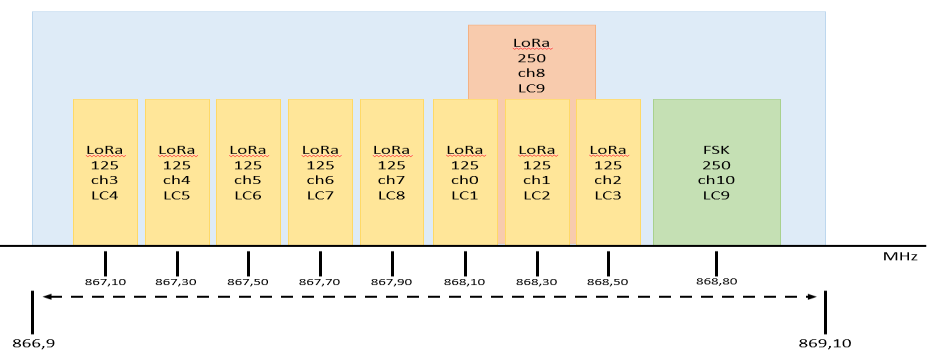
\includegraphics[width=\textwidth]{thesis.tex/chapters/context/fig/channels.png}
  \caption{LoRaWAN Channels in Europe\cite{Polonelli_2019}\label{fig:channels}}
\end{figure}

% TODO Talk about 1% duty cycle

\section{Time-Slotted Channel Hopping (TSCH)}

TSCH is a Medium Access Control (MAC) layer protocol defined by the IEEE
802.15.4e standard~\cite{rfc7554}.
The design is inherited from WirelessHART and
ISA100.11a~\cite{Duquennoy2017TSCHA6}.
Time synchronization aims to achieve low power and highly reliable
communications by using the following principles.

\begin{description}
  \item[Time-division multiple access] or (TDMA) by assigning time-slots for each
    participant in the network avoiding collisions.
  \item[Synchronization] time-synchronized nodes syncing their clock with each
    other for being able to keep the notion of time slot.
  \item[Channel Hopping] for better band usage, less interference, and more
    throughput.
\end{description}

In the following section I will present the TSCH protocol building blocks.

\subsection{Time Slots}

A time slot in TSCH is a unit of time to execute the network operations. 
The duration of the time slot is not standardized and depends on the physical 
layer we are using. 
Time slots should be long enough for the longest frame size to be sent
between two nodes, together with an acknowledgement~\cite{rfc7554}. 
Every time slot in a TSCH network has the same duration.

For each time slot operation, a schedule orchestrates what each
node of the network will use his time-slot for.

\begin{description}
  \item [Transmit] if a packet is on the outgoing buffer of the node.
  \item [Receive] listen for incoming packets that may arrive.
  \item [Sleep] to save energy.
\end{description}

Each transmitting or receiving time slot is made of the following parts.

\begin{itemize}
  \item The packet transmission or reception.
  \item Guard time for time slots synchronization.
  \item Acknowledgement reception or transmission.
\end{itemize}

\paragraph{}

A set of time slots that repeat over time is known as a slotframe.
A slotframe is made of time slots and empty slots.
The slotframe length has a direct impact on network capacity.
Figure~\ref{fig:timeslots} represent how time slots and slotframes are
organized together. 

\begin{figure}[H]
  \centering

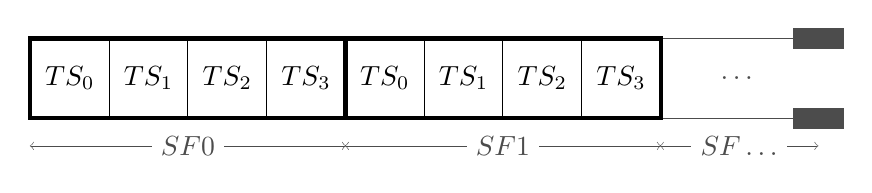
\begin{tikzpicture}[
  timeslot/.style={draw, rectangle, minimum size=1cm},
  arr/.style={help lines,black!70,<->},
]

\foreach [evaluate={\ts=int(mod(\i, 4))}] \i in {0,...,7} {
  \node (ts\i) [timeslot] at (\i, 0) {$TS_{\ts}$};
}
\node (ts8) [minimum height=1cm, minimum width=2cm, black!70] at (8.5, 0) {\ldots};
\draw[help lines, black!70]
  (ts8.north west) -- (ts8.north east) node[fill=white, black!70] {$\ldots$};
\draw[help lines, black!70]
  (ts8.south west) -- (ts8.south east) node[fill=white, black!70] {$\ldots$};

\draw[ultra thick] 
  (ts0.south west) rectangle (ts3.north east)
  (ts4.south west) rectangle (ts7.north east);

\draw[arr]
  ([yshift=-10pt]ts0.south west) -- node[fill=white] {$SF0$} ([yshift=-10pt]{ts3.south east});
\draw[arr]
  ([yshift=-10pt]ts4.south west) -- node[fill=white] {$SF1$} ([yshift=-10pt]{ts7.south east});
\draw[arr]
  ([yshift=-10pt]ts8.south west) -- node[fill=white] {$SF\ldots$} ([yshift=-10pt]{ts8.south east});

\end{tikzpicture}

\caption{Slotframes representation\label{fig:timeslots}}
\end{figure}


\subsection{Absolute Slot Number (ASN)}

The absolute slot number is a shared counter between all the devices that
define the number of time slots elapsed since the start of the
network (see Fig~\ref{fig:asn}).
ASN increases after each time-slot and is calculated with \ref{eq:asn} where $k$
is the slotframe offset.

\begin{equation}
  \label{eq:asn}
  ASN = k SF_{len} + TS_{offset}
\end{equation}

\begin{figure}[H]
\centering
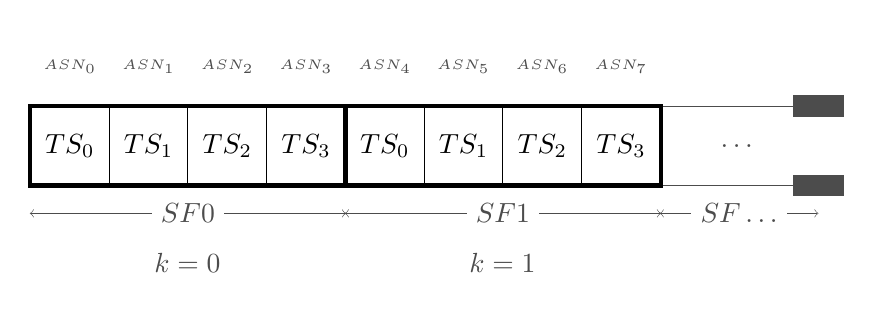
\begin{tikzpicture}[
  asn/.style={black!70, minimum size=1cm},
  timeslot/.style={draw, rectangle, minimum size=1cm},
  arr/.style={help lines,black!70,<->},
  desc/.style={black!70},
]

\foreach \i in {0,...,7} {
  \node (ts\i) [asn] at (\i, 1) {\tiny $ASN_{\i}$};
}
\foreach [evaluate={\ts=int(mod(\i, 4))}] \i in {0,...,7} {
  \node (ts\i) [timeslot] at (\i, 0) {$TS_{\ts}$};
}
\node (ts8) [minimum height=1cm, minimum width=2cm, black!70] at (8.5, 0) {\ldots};
\draw[help lines, black!70]
  (ts8.north west) -- (ts8.north east) node[fill=white, black!70] {$\ldots$};
\draw[help lines, black!70]
  (ts8.south west) -- (ts8.south east) node[fill=white, black!70] {$\ldots$};

\draw[ultra thick] 
  (ts0.south west) rectangle (ts3.north east)
  (ts4.south west) rectangle (ts7.north east);

\draw[arr]
  ([yshift=-10pt]ts0.south west) -- node[fill=white] {$SF0$} ([yshift=-10pt]{ts3.south east});
\draw[arr]
  ([yshift=-10pt]ts4.south west) -- node[fill=white] {$SF1$} ([yshift=-10pt]{ts7.south east});
\draw[arr]
  ([yshift=-10pt]ts8.south west) -- node[fill=white] {$SF\ldots$} ([yshift=-10pt]{ts8.south east});
\node[desc] at
  ([xshift=2cm, yshift=-28pt]ts0.south west) {$k = 0$};
\node[desc] at
  ([xshift=2cm, yshift=-28pt]ts4.south west) {$k = 1$};
\end{tikzpicture}
\caption{Absolute Slot Number\label{fig:asn}}
\end{figure}


\subsection{Channel Hopping}

\emph{Channel Hopping} increases the network capacity with frequency diversity
to mitigate interferences.
Multiple device can share time-slots to transmit at the same time on different
channels.

Links are the conjunction of a time slot and a channel~\cite{Chen2013PerformanceAO}.

\begin{equation}
  \label{eq:links}
  link = (TimeSlot_{number}, Channel_{offset})
\end{equation}

Multiple links constitute a time slot (dependent on the number of channels
available). Devices can transmit on different links during the same time slot.

% TODO Topology example multiple timeslot same time TX on different channels

The channel offset is computed by the transmitter and the receiver with the
function~\ref{eq:channel}. Both nodes know the $ASN$ and the schedule and can
compute the same channel offset~\cite{rfc7554}.

\begin{equation}
  \label{eq:channel}
  Channel_{offset} = (ASN + Scheduled_{offset}) \% Channel_{number}
\end{equation}

If the slotframe length is a prime number, even with the static schedule,
with known channel offset, the time slot will use a different channel every time.
Figure~\ref{fig:channelhopping} shows how scheduled cells in a TSCH network of
four time slot and three channels change channel depending on the ASN.

\begin{figure}[H]
\centering
\begin{tikzpicture}[
  asn/.style={black!70, minimum size=1cm},
  timeslot/.style={draw, rectangle, minimum size=1cm},
  arr/.style={help lines,black!70,<->},
  desc/.style={black!70},
]

\foreach \i in {0,...,7} {
  \node (asn\i) [asn] at (\i, 4) {\tiny $ASN_{\i}$};
}
\foreach [evaluate={\ts=int(mod(\i, 4))}] \i in {0,...,7} {
  \node (ts3\i) [timeslot] at (\i, 3) {};
}
\foreach [evaluate={\ts=int(mod(\i, 4))}] \i in {0,...,7} {
  \node (ts2\i) [timeslot] at (\i, 2) {};
}
\foreach [evaluate={\ts=int(mod(\i, 4))}] \i in {0,...,7} {
  \node (ts1\i) [timeslot] at (\i, 1) {};
}
\foreach [evaluate={\ts=int(mod(\i, 4))}] \i in {0,...,7} {
  \node (ts\i) [asn] at (\i, 0) {$TS_{\ts}$};
}
% \node (ts8) [minimum height=1cm, minimum width=2cm, black!70] at (8.5, 0) {\ldots};
% \draw[help lines, black!70]
%   (ts8.north west) -- (ts8.north east) node[fill=white, black!70] {$\ldots$};
% \draw[help lines, black!70]
%   (ts8.south west) -- (ts8.south east) node[fill=white, black!70] {$\ldots$};

\node (choff3) [black!70] at (-1.5, 3) {$Ch_{off} 2$};
\node (choff2) [black!70] at (-1.5, 2) {$Ch_{off} 1$};
\node (choff1) [black!70] at (-1.5, 1) {$Ch_{off} 0$};

\begin{scope}[on background layer]
\fill[blue!50] (ts10.south west) rectangle (ts10.north east);
\fill[blue!50] (ts24.south west) rectangle (ts24.north east);

\fill[orange!50] (ts30.south west) rectangle (ts30.north east);
\fill[orange!50] (ts14.south west) rectangle (ts14.north east);

\fill[green!50] (ts22.south west) rectangle (ts22.north east);
\fill[green!50] (ts36.south west) rectangle (ts36.north east);
\end{scope}

\draw[ultra thick] 
  (ts10.south west) rectangle (ts33.north east)
  (ts14.south west) rectangle (ts37.north east);

\draw[arr]
  ([yshift=-10pt]ts0.south west) -- node[fill=white] {$SF0$} ([yshift=-10pt]{ts3.south east});
\draw[arr]
  ([yshift=-10pt]ts4.south west) -- node[fill=white] {$SF1$} ([yshift=-10pt]{ts7.south east});
\draw[arr]
  ([yshift=-10pt]ts8.south west) -- node[fill=white] {$SF\ldots$} ([yshift=-10pt]{ts8.south east});
\node[desc] at
  ([xshift=2cm, yshift=-28pt]ts0.south west) {$k = 0$};
\node[desc] at
  ([xshift=2cm, yshift=-28pt]ts4.south west) {$k = 1$};
\end{tikzpicture}
\caption{Two slotframes with scheduled cells changing channel between slotframes\label{fig:channelhopping}}
\end{figure}


\subsection{Scheduling}

The TSCH schedule tells each node what to do during a time slot.

Dedicated time slots cells need the following parts to be defined.

\begin{itemize}
  \item Receive or transmit.
  \item The channel offset.
  \item Address of the node to communicate with.
\end{itemize}

% Shared cells multiple nodes can transmit at the same time on the same channel.

To ensure the execution of the same slots, each transmission is an opportunity 
for the neighbor to resynchronize their clocks.
Synchronization is important to mitigate each node internal clock drift.

Time source nodes send Enhanced Beacon (EB) packets to synchronize the receiving
nodes of the network. When nodes don't resynchronize for a long period
a Keep-Alive (KA) is sent and used to adjust the drift at synchronization.

Figure~\ref{fig:sync} represents the clock drift that can occur between two
distant time slots.
As we can see the receiver will know the drift based on the moment he receives
the data and then adjusts its timeslot length to finish earlier.

\begin{figure}[H]
  \centering
  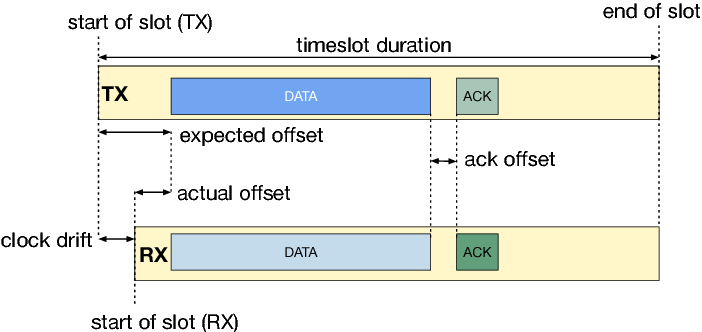
\includegraphics[width=\textwidth]{thesis.tex/chapters/context/fig/sync.png}
  \caption{Synchronization in a TSCH timeslot\cite{TELESHERMETO201784}\label{fig:sync}}
\end{figure}

\section{Contiki OS}

Contiki is a free and open-source Real-Time operating system (OS) specifically made
for IoT applications. Contiki ships with a low-power IPv6 communication stack
and a variety of routing and MAC protocols making the OS particularly well
suited for Wireless Sensor Networks (WSN).

Contiki uses protothreads, a programming abstraction which Contiki is
built around.
They allow developers to write event-driven programs with little memory overhead and
claims to reduce the complexity of embedded programs that used to be written 
like state machines~\cite{10.1145/1182807.1182811}.

The Contiki OS project has been unmaintained since 2017 but its
successor named Contiki-NG was created as a fork by the same developers since.
That fork has been the basis for a lot of LPWAN experimentation, for example 
with the development of the 6TiSCH stack for the OS~\cite{Duquennoy2017TSCHA6}.

\paragraph{}

Contiki's Network Protocol stack, also known as \lstinline{NETSTACK}, is a
feature of the OS.
It allow developers to defines parts of the network stack we are using in a Contiki
project (Fig~\ref{fig:netstack}).

NETSTACK implementation allows Contiki to communicate between layers without 
knowing the specific implementation of the layer.
Developers must define the following variables to change the network stack 
in a Contiki project.

\begin{itemize}
  \item \lstinline{NETSTACK_NETWORK}
  \item \lstinline{NETSTACK_ROUTING}
  \item \lstinline{NETSTACK_MAC}
  \item \lstinline{NETSTACK_RADIO}
\end{itemize}

\begin{figure}[H]
\centering
  \begin{tikzpicture}[->,>=stealth',shorten >=1pt,auto,node distance=1.4cm]

  \tikzstyle{comment}=[
    right=2pt,
    font=\small,
    fill=white,
    text=black,
    draw=black,
  ]

  \tikzstyle{every state}=[rectangle,thick,
    draw=black,fill=gray!20,text=black,
    minimum width= 6cm,
    minimum height= 1.20cm
  ]

  \tikzstyle{smallstate}=[rectangle,thick,
    draw=black,fill=gray!10,text=black,
    minimum width= 4cm,
    minimum height= 1.20cm
  ]

  \node[smallstate]         (A)                    {Network Layer};
  \node[smallstate]         (B) [below of=A]       {Routing};
\begin{scope}[on background layer]
  \node[state, fit=(A)(B)] (AB)                 {};
\end{scope}
  \node[state,below=1cm]         (C) [below of=AB]       {MAC Layer};
  \node[state]         (D) [below of=C]       {Physical Layer};

  \node[comment]       at (AB.north west) {Network Layer};
  % \node[comment]       at (C.north west) {MAC Layer};
  % \node[comment]       at (D.north west) {Physical Layer};
  % \path (A) edge [bend right]    node {     } (B)
  %           edge [bend left]     node {     } (C)
  %       (B) edge [bend left]     node {     } (C)
  %           edge                 node {     } (D)
  %       (C) edge [bend left]     node {     } (A)
  %       (D) edge [bend right=85] node {     } (A);
\end{tikzpicture}
\caption{The Contiki's Network Protocol Stack\label{fig:netstack}}
\end{figure}


\section{Routing}

\section{Related work}

This is not the first attempt to bring multi-hop communication to LoRa.
This section will give a state of the art of the research on
multi-hop routing in LoRa.

\paragraph{}

Work to port TSCH and the 6LoWPAN stack to a new radio protocol has already 
been done in~\cite{uwbtsch} for the Ultra-Wide Band (UWB).

% \paragraph{BLEach}

\paragraph{UWB-TSCH}

Charlier M. in~\cite{uwbtsch} explores the requirements to adapt TSCH for the UWB.
Similarly to LoRa, UWB does not allow CCA and can not use CSMA for its 
communications.
His work shows what it takes to adapt TSCH for another radio layer. 
It is also an evaluation of the performance of TSCH outside of 802.15.4.

\paragraph{}

The respective authors of~\cite{DIAS2018424, 8856256}, look at ways to extend
the current LoRaWAN MAC protocol to allow multi-hop communications.

\paragraph{Multihop LoRaWAN Extension} Dias J., Grilo A. in \cite{DIAS2018424}
design a routing protocol that can interoperate with LoRaWAN gateways while
using multi-hop communications for nodes out of the range of the gateway.  
The extension uses beacons to achieve time synchronization, but no channel
hopping is used.

% \paragraph{Distributed Queuing (DQ) LoRa}

% The authors of~\cite{8856256} extend LoRaWAN

% \subsection{RS LoRa}
% [18] in roald similar to lorawan extension
% \subsection{Listen before talk LoRa}
% [17] in roald work

\paragraph{}

Studies on creating a new MAC protocol for multi-hop LoRa communications in a linear
network has been done in~\cite{Abrardo_2019,duong2018}.

\paragraph{Linear Multihop LoRa}

Abrardo A. and Pozzebon A.~\cite{Abrardo_2019} studied the deployment of a
large scale LoRa network to monitor the underground medieval aqueducts of the city center 
of Sienna, the \emph{Bottini}.

Because of the large deployment cost induced by the large tunnels, the negative 
aesthetic impact of a wired network and the risk of flooding, made the author
opt for a battery-operated wireless network.


They propose a multi-hop routing solution for Linear Sensor Network (LSN) based 
on LoRa by developing their own MAC protocol tailored for their scenario.
This custom protocol is built around assigning time slots for each node with
a common schedule for adjacent nodes.
This allows neighbors to synchronize their clock and broadcast messages to
both ends of the aqueducts.

% Their solution allowed the connection of the Bottini

\paragraph{Multi-Hop Linear Network Based on LoRa}

Duong T. in~\cite{duong2018} proposes a multi-hop protocol for LoRa linear
networks. 
His network is made of two periods. The first is the network initialization to
verify the gateway is reachable and synchronizes the nodes to make them join the 
data operation period.
Each node transmits in a different timeslot to their parent node, each hop adds
their information to the packet they are relaying until the gateway is
reached.
The clock drift is mitigated by synchronizing on the preamble but the receiver
does not acknowledge the reception of the packet, making the network sensible to
interference since it is running on a single channel and SF.

\paragraph{}

The next studies look at ways to create a fully functioning multi-hop network
using LoRa without depending on LoRaWAN specifications.

\paragraph{LoRaBlink}

Bor M., Vidler J., Roedig Utz. in \cite{lorablink} propose the LoRaBlink
protocol, designed to support reliable and energy efficient multi-hop
communication.

Each node of the network remains in listening mode until a beacon is received.
Beacons are used for time synchronization of the time slots.
Each node transmit packets to their parent node that relays it to the gateway.
There is no scheduling of which node transmits, two nodes may
transmit at the same time.

% Every nodes of the network keep track of their distance to the sink

Also, LoRaBlink uses fixed SF, BW, and channel. This decreases the overall throughput 
of the network and makes it highly sensitive to interference.

\paragraph{RPL+LoRa MAC Protocol}

The Authors of~\cite{8115756} from the SmartNet research group of VUB, adapted RPL 
to enable multihop communications on top of LoRa. 
The paper presents the modifications of the objective function to take into
account the SF when computing the best routes.
The paper describes a solution for a network of nodes to discover each other.
It uses a router sending packets on different spreading factors while the joining
node listens on the spreading factors by starting by the lowest, this way it
picks the fastest spreading factor available.
It also describes a custom MAC protocol, \emph{RLMAC}, to allow multi-hop
routing with LoRa. It manages time-slots between nodes and allows PHY settings
tuning depending on the links.

The protocol proposed focused on having the fastest delivery time with LoRa
communications while increasing the packet delivery rate (PDR).
Reducing the power consumption was not a concern in this paper.


\paragraph{TSCH-over-LoRa}

In the course of my work, a new study from Haubro M., Orfanadis C.,
Oikonomou G. and Fafoutis X.~\cite{tschoverlora} came out on the exact 
same subject as mine. 
Their work studied the feasibility of porting TSCH to LoRa in Contiki OS using
SX1272 radio module.

The authors proved it was possible to adapt TSCH for LoRa by testing their
implementation with a variety of routing protocols and applications.
Their implementation works on a single SF at a time but they tested it using
SF7 and SF10.

To demonstrate the resilience of TSCH to interference even with LoRa, the
authors made a radio jammer that transmits on different channels. Their
experimentation proved no packets got lost when using channel hopping with
LoRa.
